\begin{center}
\begin{tikzpicture}
	\node[anchor=south west,inner sep=0] (image)  at (0,0) {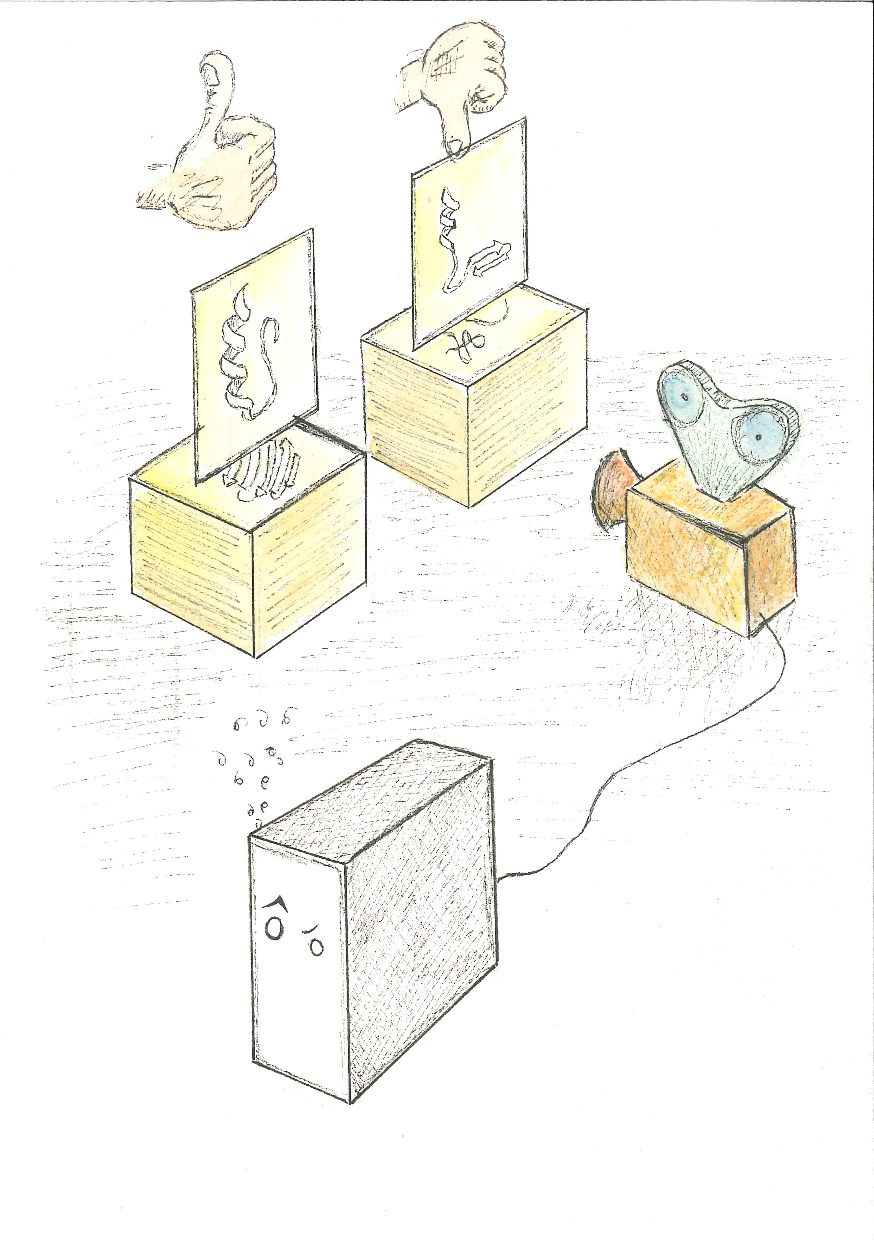
\includegraphics[trim={2mm, 2mm, 2mm, 2mm}, width=0.995\pagewidth]{scans/pan-2.pdf}};
    \begin{scope}[x={(image.south east)},y={(image.north west)}]
		\if\helplines1
			\draw[help lines,xstep=.1,ystep=.1] (0,0) grid (1,1);
		\else
			\path[help lines,xstep=.1,ystep=.1] (0,0) grid (1,1);
		\fi
		\node[text width=0.34\pagewidth, align=justify, anchor=north east] at (1-0.03, 0.95) {\english{The last step is evaluating the quality of the models. We try to teach a computer to do this by showing it many models, good and bad, and asking it to learn the differences. This is called \emph{machine learning}.}};
		
		\node[text width=0.32\pagewidth, align=justify, anchor=north east] at (1-0.06, 0.28) {\spanish{El último paso es evaluar la calidad de los modelos. Intentamos enseñar al ordenador a hacerlo por nosotros mostrándole modelos, buenos y malos, y pidiéndole que aprenda las diferencias. Se llama \emph{aprendizaje automático}.}};
    \end{scope}

\end{tikzpicture}
\end{center}
